\documentclass[12pt]{article}

\usepackage{minted}
\usepackage{hyperref}
\usepackage{datetime}
\usepackage{datenumber}
\usepackage{pdfpages}
\usepackage{advdate}
\usepackage[super]{nth}
\usepackage[margin=0.75in]{geometry}

\parindent 0pt \parskip 6pt


\begin{document}

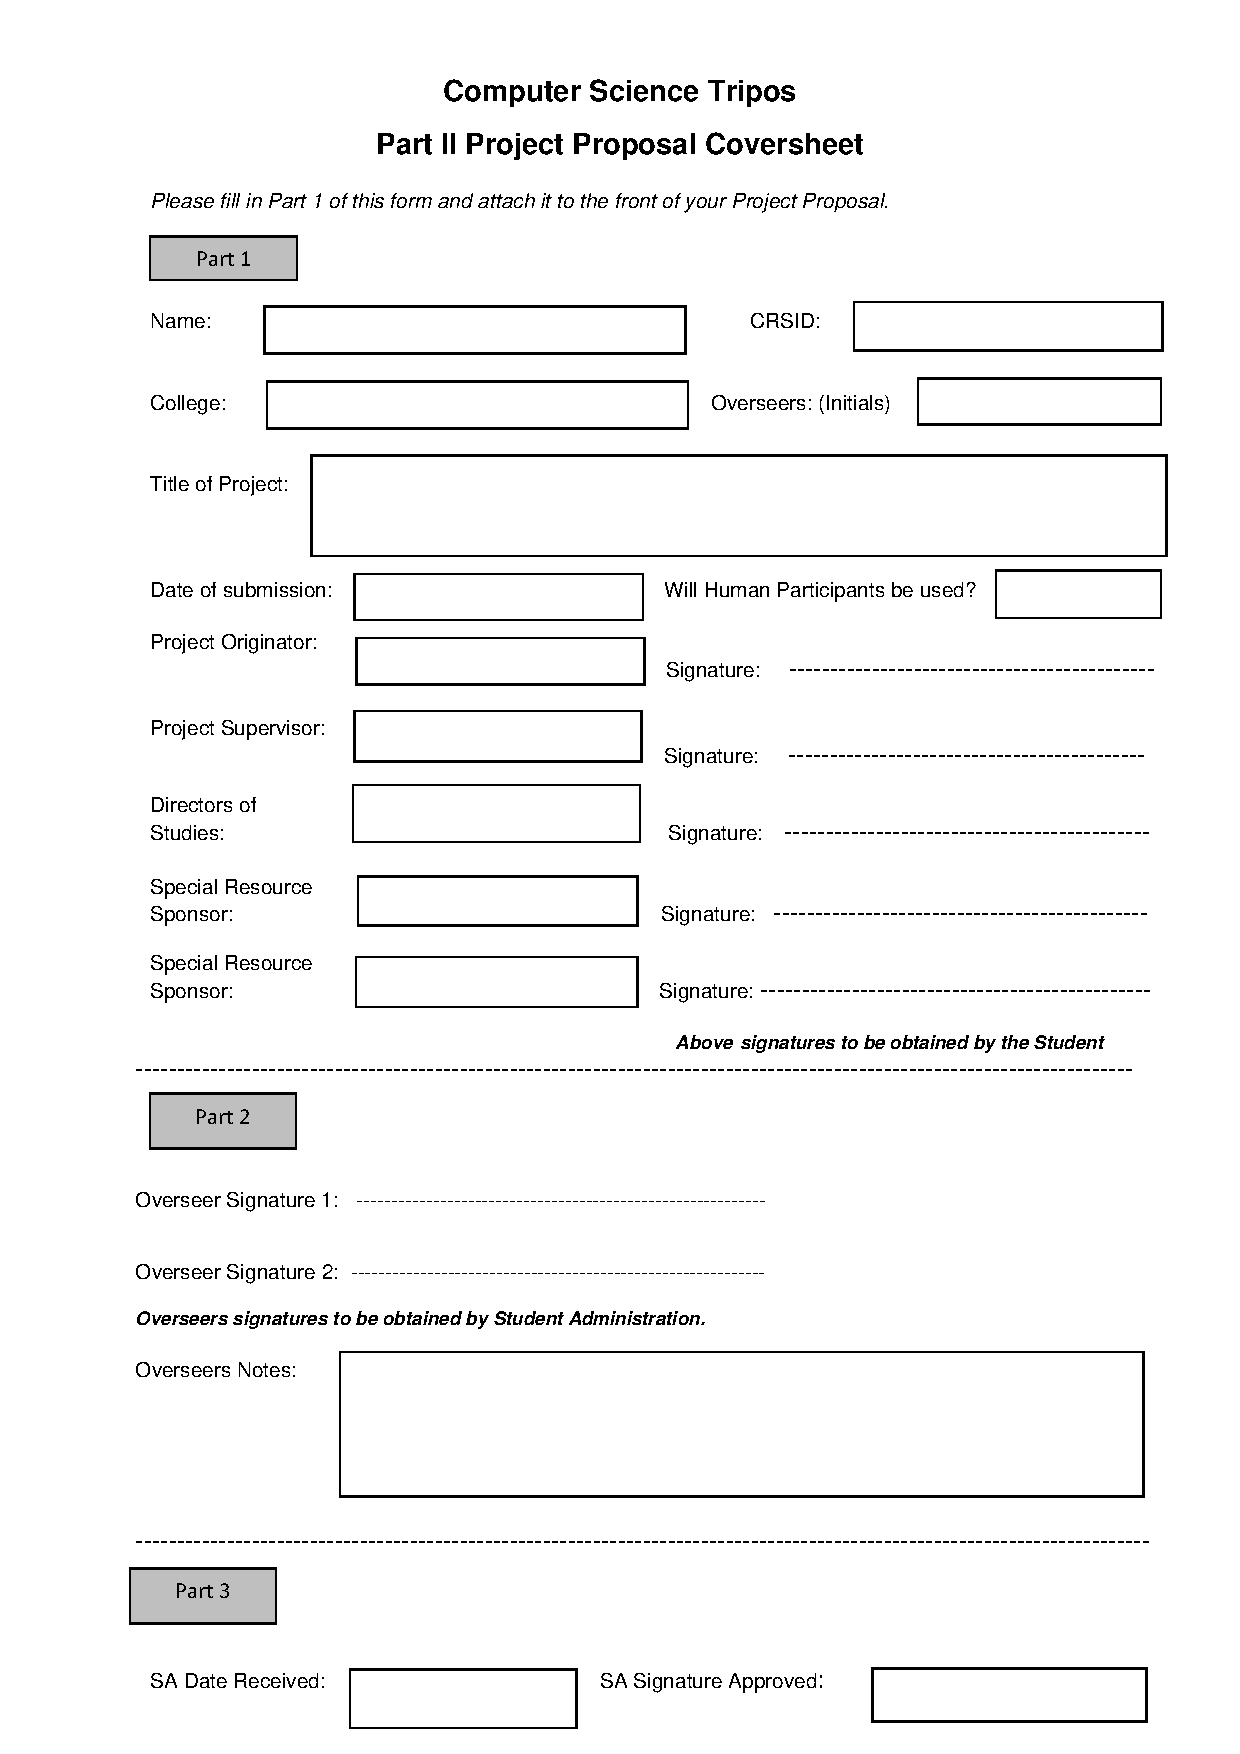
\includepdf[pages={1}]{ProposalForm.pdf}

\thispagestyle{empty}

\centerline{\large Computer Science Tripos: Part II Project Proposal}
\vspace{0.4in}
\centerline{\Large\bf Measuring mutual information within Neural networks}
\vspace{0.3in}

\centerline{Andrius Grabauskas, ag939}
\centerline{Robinson College}

\centerline{\large \textbf{\today}}

\vspace{1in}

\begin{tabular}{ p{4cm} p{4.5cm} l }
{\bf Project Originator:} & Andrius Grabauskas & \\[3mm]
{\bf Project Supervisor:} & Dr.\ Damon Wischik \\[3mm]
{\bf Director of Studies:} & Prof.\ Alan Mycroft \\[3mm]
{\bf Overseers:} & Dr.\ Robert Mullins & Prof.\ Pietro Lio' \\[3mm]
\end{tabular}

\vspace{0.75in}

\section*{Introduction and Description of the Work}

The goal of this project is to confirm or deny the results produced by
Shwartz-ziv \& Tishby in their paper ``Opening the black box of Deep Neural
Networks via Information``\footnote{https://arxiv.org/abs/1703.00810}

The paper tackles our understating of Deep Neural Networks (DNN`s). As of yet
there is no comprehensive theoretical understanding of how DNN`s learn from data.
The authors proposed to measure how information travels within the DNN`s layers.

They found that training of neural networks can be split into to two distinct
phases: memorization followed by the compression phase.
\begin{itemize}
  \item memorization - each layer increases information about the input and the
    label
  \item compression  - this is the generalization stage where each layer tries
    to forget details about the input while still increasing mutual information
    with the label thus improving performance of the DNN. This phase takes the
    wast majority of the training time.
\end{itemize}

They found that each layer in neural network tries to throw out unnecessary data
from the input while preserving information about the output/label. As the
network is trained each layer preserves more information about the label

The results they found were interesting but also contentious as they have not
yet provided a formal proof, just experimental data as a result there are many
peers that are cautious and sceptical of the theory even a
paper\footnote{https://openreview.net/pdf?id=ry\_WPG-A-} was produced that tries
to suggest that the theory is wrong, however this was dismissed by Tishby \&
Shwartz-Ziv\footnote{https://openreview.net/forum?id=ry\_WPG-A-\&noteId=S1lBxcE1z}


\section*{Starting Point}

I have watched a talk that Prof.\ Tishby gave on this topic at Yandex, no other
preparation was done. 

\section*{Resources Required}

The training of DNN`s will be computationally expensive so I will be using Azure
cloud GPU service to acquire the required compute for this project. The GPU
credits will be provided by Damon Wischik

For backups I intend to store my work on GitHub and my own personal machine. In
case my laptop breaks I will get another one or use the MCS machines.

\section*{Substance and Structure of the Project}

The aim of this project to reproduce the results provided by Prof.\ Tishby and
his colleagues. The intention of my work is to help settle the debate surrounding the
topic either strengthening the arguments in favour of the theory in case my
results are inline with the aforementioned results or encourage discussion in
case my results contradict the theory.

My work will require me to have a comprehensive understanding of Information
theory, Information bottleneck and neural networks.

One of the more contentious parts of my project will be measuring mutual
information between the input a layer in the DNN and the label. It will be
computationally expensive to measure it in DNN since we will need to retrain the
network in order to get a distribution rather than a single value. I will use
Gaussian approximation to measure it (relevant
paper\footnote{https://arxiv.org/abs/1508.00536})

Will need to use Python to train the neural networks and GNUplot or alternative
to plot the results.

\section*{Success Criteria}

Reimplement the code that was used to generate the papers results. Confirm or
deny the results produced in``Opening the black box of Deep Neural Networks via
Information`` paper on the same dataset as the paper. In order to do that I will
need to: Train a neural network on the same dataset that was used in the paper
and measure mutual information between the layers. Analyse the results produced
and address any discrepancies that may have occurred.

\section*{Extensions}

Provided I achieve the success criteria there are two main ways to extend it.

\begin{itemize}
  \item {
      Use different datasets to test the theory. Using different datasets would
      confirm that the results are not dataset specific. Current datasets we
      considered are MNIST\footnote{http://yann.lecun.com/exdb/mnist/} and
      NOT-MNIST\footnote{https://www.kaggle.com/quanbk/notmnist}.
  }
  \item {
      Explore different ways of measuring mutual information. One interesting
      way would be to explore a discrete neural network where every node would
      only be able assigned discrete values say {1...256} this would make
      measuring mutual information more defined, however this would possibly
      hurt the performance of the whole network.
  }
\end{itemize}

\section*{Schedule}

% Set start date to 15th October 2018
\ThisYear{2018}\ThisMonth{10}\ThisDay{20}

% Specify date format like "15th Oct"
\newdateformat{datefmt}{\nth{\THEDAY} \shortmonthname[\THEMONTH]}

% Force advdate commands to change the global "today" instance, not the local one
\makeatletter
\renewcommand\AdvanceDate[1][\@ne]{\global\advance\day#1 \FixDate}
\renewcommand\FixDate{%
  \FixMonth \is@LeapYear
  \l@@p \global\ifnum\day<1 \Pr@vD@y \repeat
  \l@@p \M@s\m@sic \global\ifnum\day>\M@s \N@xtD@y \repeat
}
\renewcommand\FixMonth{%
  \L@@p \global\ifnum\month<1 \global\advance\year\m@ne \global\advance\month12 \is@LeapYear \repeat
  \L@@p \global\ifnum\month>12 \global\advance\year\@ne \global\advance\month-12 \is@LeapYear \repeat}
\def\Pr@vD@y{%
  \global\ifnum\day<-366
    \global\ifnum\month>2
      \global\advance\day\r@k \global\advance\year\m@ne \is@LeapYear
    \else
      \global\advance\year\m@ne \is@LeapYear \advance\day\r@k
    \fi
  \else
    \global\advance\month\m@ne \FixMonth
    \global\advance\day\m@sic
  \fi}
\def\N@xtD@y{%
  \global\ifnum\day>366
    \global\ifnum\month>2
      \global\advance\year\@ne \is@LeapYear \global\advance\day-\r@k
    \else
      \global\advance\day-\r@k \global\advance\year\@ne \is@LeapYear
    \fi
  \else
    \global\advance\day-\M@s \global\advance\month\@ne \FixMonth
  \fi}
\makeatother

% Output eg. boldface "15th Oct - 29th Oct" when called.
\newcommand{\daterange}[1]{%
    \textbf{\datefmt\today}
    \textbf{--}
    \AdvanceDate[#1]\relax
    \AdvanceDate[-1]\relax
    \textbf{\datefmt\today}
    \AdvanceDate[1]\relax
}

\begin{itemize}
  \item {
      \daterange{14}

      I expect to spend the first week reading up on Information theory
      (primarily from Mackay`s book\footnote{Informaition Theory, Inference, and
      Learning Algorithms by David J. C. MacKay}) and the information bottleneck
      method in order to understand the nuances of the paper.
  }
  \item {
      \daterange{28}
      
      The following weeks I intend to spend reading up on DNN`s doing some
      introductory courses, I will train the neural network on the same data as
      the paper but at this point will not yet try to measure the mutual
      information between the layers.

      At this point I will also start examining the
      code\footnote{https://github.com/ravidziv/IDNNs} provided and start to
      implement parts of it which don't deal with information measurement.
  }
  \item {
      \daterange{28}

      Will start reading up on mutual Information measurement with local
      Gaussian approximation.

      Implementing mutual information measurement in code.

      At this point I expect the computation to be too demanding for my machine
      and will need to use Azure.
  } 
  \item {
      \daterange{35}

      Having a working system to test data sets I will try to reproduce results
      from the paper on the same dataset. This will achieve my success criteria.

      At this point my success criteria should be completed I will spend some
      time writing the skeleton of the thesis. Look for any discrepancies
      between my results and the ones provided in the paper.
  } \item {
      \daterange{42}

      Assuming everything goes as planned I will start looking into implementing
      one of the extensions.

      Either reproducing the results on a different dataset too see if the
      results of the paper are not dataset specific. Or to implement a discrete
      DNN in order to measure mutual information in a fully defined way.
  } \item {
      \daterange{28}

      Will use the remaining time to write up the dissertation.
  }
\end{itemize}

\end{document}
